% --------------------------------------------------------------------------------

\section{Behavior of the Modern Hopfield Network}

% --------------------------------------------------------------------------------

\begin{frame}
	
\frametitle{Properties -- Network Capacity}

Larger network capacities with higher interaction vertices:
\begin{align}
    K_{\text{max}} = \frac{1}{2\left(2n-3\right)!!} \frac{N^{n-1}}{\ln(N)}
\end{align}

Notably, super-linear for \(n>2\).

\end{frame}

% --------------------------------------------------------------------------------

\begin{frame}
    \frametitle{Properties -- Training Times}

Faster training times with higher interaction vertices:
\begin{figure}
    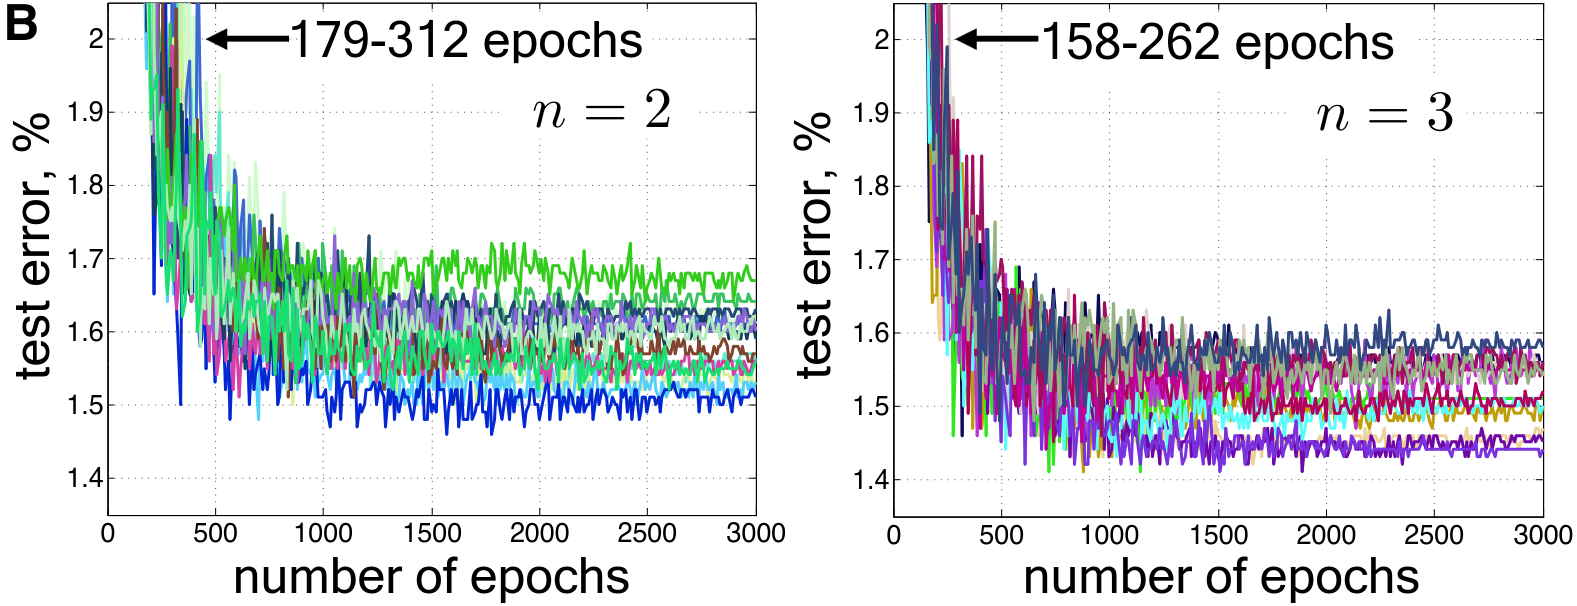
\includegraphics[width=\textwidth]{images/trainingTimes.png}
    \caption{Krotov and Hopfield 2016, Figure 01}
\end{figure}
\end{frame}

% --------------------------------------------------------------------------------

\begin{frame}
    \frametitle{Properties -- Feature to Prototype Transition}

Low interaction vertices result in memories that look like features, while higher interaction vertices result in memories that look like prototypes:

\begin{columns}
    \column{.5\textwidth}
    \begin{figure}
        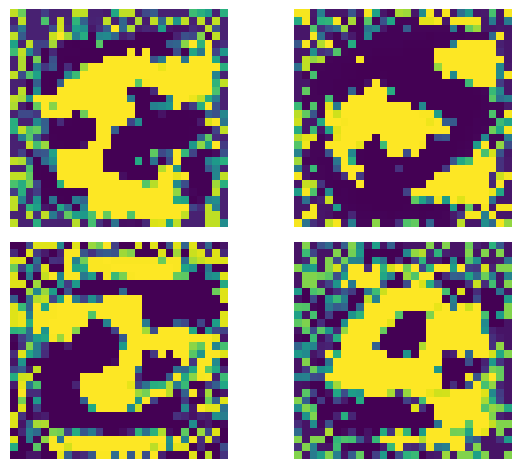
\includegraphics[width=\textwidth]{images/featureDetector.png}
    \caption{Feature-like Memories, \(n=2\)}
    \end{figure}
    \column{.5\textwidth}
    \pause
    \begin{figure}
    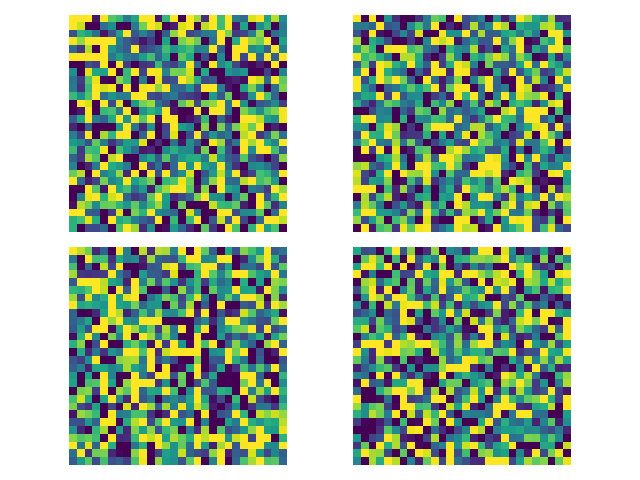
\includegraphics[width=\textwidth]{images/randomMemories/00.png}
    \caption{Prototype-like Memories, \(n=20\)}
    \end{figure}
    % \only<1>{
    %     \begin{figure}
    %     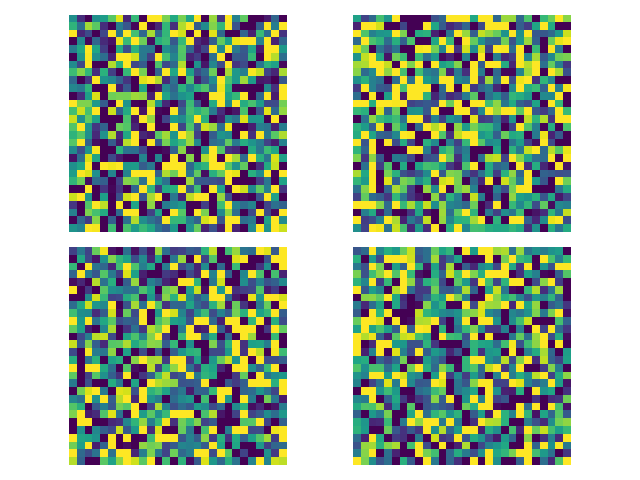
\includegraphics[width=\textwidth]{images/randomMemories/01.png}
    %     \caption{Prototype-like Memories, \(n=20\)}
    %     \end{figure}
    % }
    % \only<2>{
    %     \begin{figure}
    %     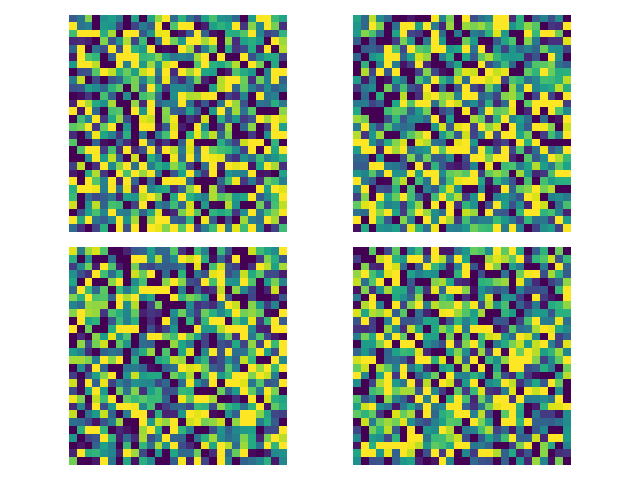
\includegraphics[width=\textwidth]{images/randomMemories/02.png}
    %     \caption{Prototype-like Memories, \(n=20\)}
    %     \end{figure}
    % }
    % \only<3>{
    %     \begin{figure}
    %     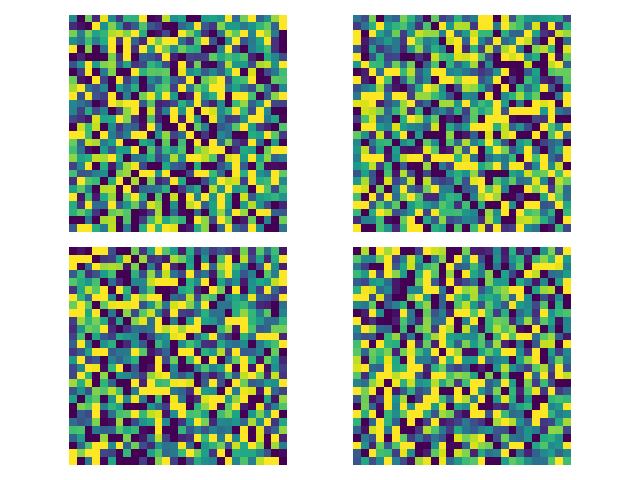
\includegraphics[width=\textwidth]{images/randomMemories/03.png}
    %     \caption{Prototype-like Memories, \(n=20\)}
    %     \end{figure}
    % }
    
\end{columns}

\end{frame}


% \begin{frame}
%     \frametitle{Why is our implementation broken?}

%     \begin{itemize}
%         \item Other implementations online\dots
%         \begin{itemize}
%             \item Most use a feed-forward architecture that isn't as general.
%             \item An example of the autoassociative memory exists, and works!
%             \item When translated line by line to PyTorch, still broken\dots
%         \end{itemize}
%         \item Hyperparameters are numerous and ``magic''.
%     \end{itemize}
% \end{frame}